\section{Introduction}\label{sec:Introduction}



Large language models (LLMs)~\cite{wei2022emergent,gpt3-brown2020language,chowdhery2022Palm,openai2022gpt4techreport,kaplan2020scalinglaws} have shown impressive abilities in a wide variety of tasks spanning natural language processing, question answering, code generation, etc. This has led to tremendous increase in their usage across many applications such as chatbots~\cite{openai2022gpt4techreport,chatgpt,claudeai,characterai}, search~\cite{bingai,komoai,youdotcom,perplexityai,bard}, code assistants~\cite{githubcopilot,replitghostwriter,amazoncodewhisperer}, etc. The significant GPU compute required for running inference on large models, coupled with significant increase in their usage, has made LLM inference a dominant GPU workload today. Thus, optimizing LLM inference has been a key focus for many recent systems~\cite{efficiently-scaling-transformer-inference,flexgen,orca,vllmsosp,patel2023splitwise,distserve2024,sarathi2023}.

\begin{figure}
    \begin{subfigure}[b]{0.235\textwidth}        
        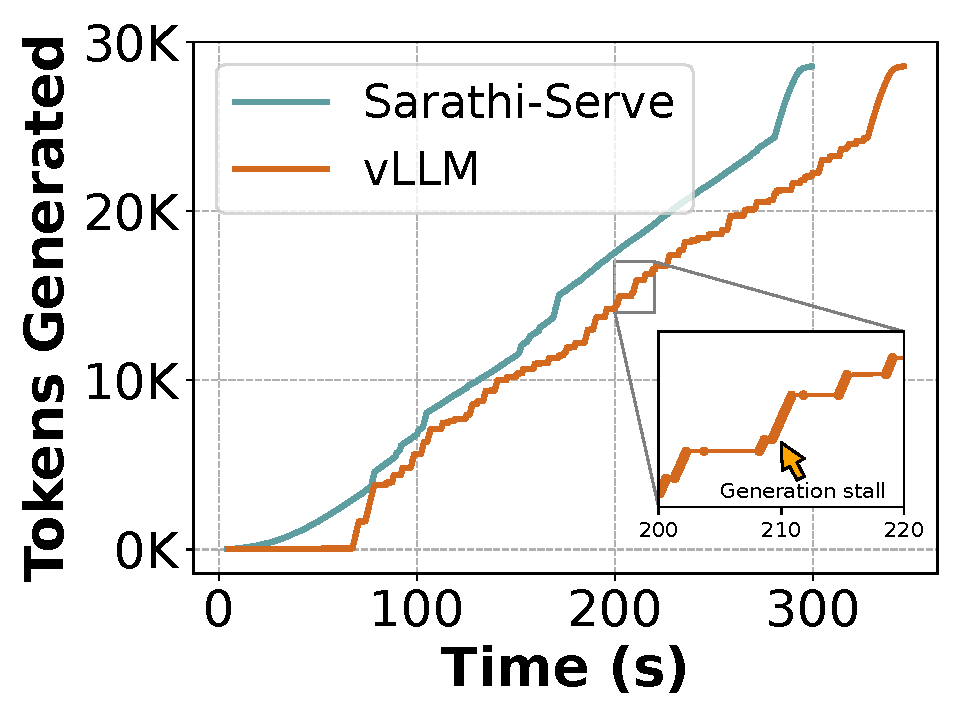
\includegraphics[ width=\textwidth]{figures/yi-arxiv-banner.pdf}
        \caption{Generation stall.}
        \label{fig:banner:stal}
    \end{subfigure}
    \begin{subfigure}[b]{0.23\textwidth}
        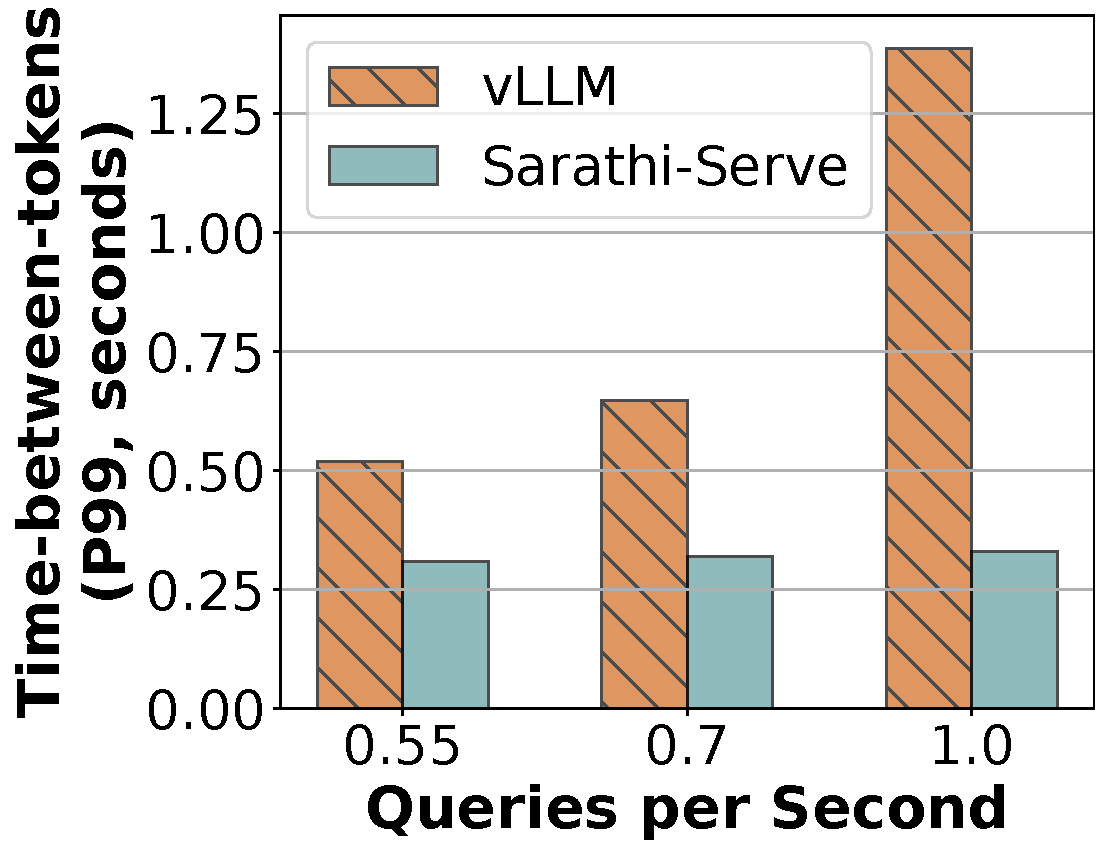
\includegraphics[width=\textwidth]{figures/banner-latency.pdf}
        \caption{High tail latency.}
        \label{fig:banner:latency}
    \end{subfigure}
    \caption{
    \yi running on two A100 GPUs serving 128 requests from \textit{arxiv-summarisation} trace. ~\ref{fig:banner:stal} highlights one of the many generation stalls lasting over several seconds in vLLM ~\cite{vllmsosp}. ~\ref{fig:banner:latency} shows the impact of increasing load on tail latency. \sysname improves throughput while eliminating generation stalls.}
    \vspace{-1em}
\end{figure}


Optimizing throughput and latency are both important objectives in LLM inference since the former helps keep 
serving costs tractable while the latter is necessary to meet application requirements. In this paper, we show that current LLM serving systems have to face a tradeoff between throughput and latency. In particular, LLM inference throughput can be increased significantly with batching. However, the way existing systems batch multiple requests leads to a compromise on either throughput or latency. For example,~\autoref{fig:banner:latency} shows that increasing load can significantly increase tail latency in a state-of-the-art LLM serving system vLLM ~\cite{vllmsosp}.


Each LLM inference request goes through two phases -- a \textit{prefill} phase followed by a \textit{decode} phase. The \textit{prefill} phase corresponds to the processing of the input prompt and the \textit{decode} phase corresponds to the autoregressive token generation. The prefill phase is compute-bound because it processes all tokens of an input prompt in parallel whereas the decode phase is memory-bound because it processes only one token per-request at a time. Therefore, decodes benefit significantly from batching because larger batches can use GPUs more efficiently whereas prefills do not benefit from batching.


Current LLM inference schedulers can be broadly classified into two categories\footnote{We classify recent schedulers Splitwise~\cite{patel2023splitwise} and DistServe~\cite{distserve2024} under a third category ``disaggregated'' and discuss them in~\autoref{section:relatedwork}.}, namely, 
\prefillprio and \decodeprio depending on how they schedule the prefill and decode phases while batching requests. In this paper, we argue that  both strategies have fundamental pitfalls that make them unsuitable for serving online inference (see~\autoref{fig:intro:tradeoff-space}).



Traditional request-level batching systems such as FasterTransformer~\cite{fastertransformer} employ \decodeprio scheduling. These systems submit a batch of requests to the execution engine that first computes the prefill phase of all requests and then schedules their decode phase. The batch completes only after all requests in it have finished their decode phase i.e., new prefills are not scheduled as long as one or more requests are doing decodes. This strategy optimizes inference for latency metric time-between-tokens or TBT -- an important performance metric for LLMs. This is because new requests do not affect the execution of ongoing requests in their  decode phase. However, \decodeprio schedulers severely compromise on throughput because even if some requests in a batch finish early, the execution continues with reduced batch size until the completion of the last request. 



\begin{figure}[t!]
    \centering
        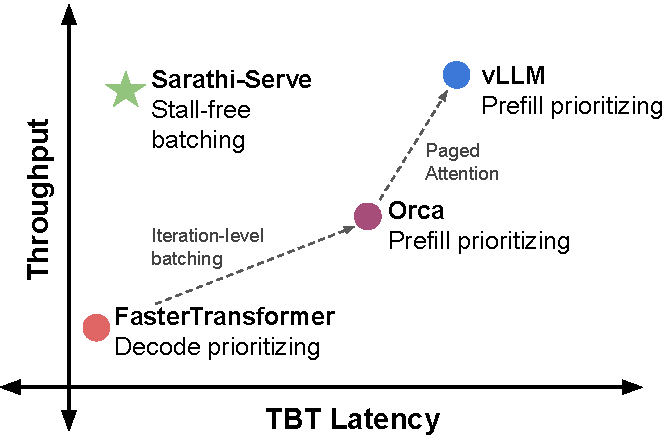
\includegraphics[width=0.4\textwidth]{figures/tradeoff_space.pdf}

    \caption{ Current LLM serving systems involve a tradeoff between throughput and latency depending on their scheduling policy. Prioritizing prefills optimizes throughput but sacrifices TBT (time-between-tokens) tail latency whereas prioritizing decodes has the opposite effect. \sysname serves high throughput with low TBT latency via stall-free batching. (The figure is illustrative and actual values will depend on the model and workload characteristics.)}
       \label{fig:intro:tradeoff-space}
\end{figure}



Orca~\cite{orca} introduced iteration-level batching wherein requests can dynamically enter or exit a batch at the granularity of individual iterations. Iteration-level batching improves throughput by avoiding inefficiencies of request-level batching systems. Orca and several other recent systems like vLLM~\cite{vLLM:github} combine iteration-level batching with \prefillprio scheduling wherein they eagerly schedule the prefill phase of one or more requests first i.e., whenever GPU memory becomes available. This way, \prefillprio schedulers have better throughput because computing prefills first allows subsequent decodes to operate at high batch sizes. However, prioritizing prefills leads to high latency because it interferes with ongoing decodes. Since prefills can take arbitrarily long time depending on the lengths of the given prompts, \prefillprio schedulers lead to an undesirable phenomenon that we refer to as \textit{generation stalls} in this paper. For example, ~\autoref{fig:banner:stal} shows that a generation stall in vLLM can last over several seconds.

Another challenge introduced by traditional iteration-level scheduling systems like Orca~\cite{orca} is pipeline stalls or bubbles~\cite{gpipe}. These appear in pipeline-parallelism (PP) deployments that are needed to scale LLM inference across several nodes. In servers with high bandwidth connectivity such as NVIDIA DGX A100~\cite{nvidiadgx}, tensor-parallelism (TP)~\cite{megatron} can enable deployment of an LLM on up to 8 GPUs,  supporting large batch sizes with low latencies. However, TP can have prohibitively high latencies when hyper-clusters are unavailable~\cite{varuna}. Thus, as an alternative to TP, pipeline-parallelism (PP)~\cite{pipedream, varuna} is typically used across commodity networks. Existing systems rely on micro-batches to mitigate pipeline stalls or bubbles~\cite{gpipe}. However, the standard micro-batch based scheduling can still lead to pipeline bubbles due to the unique characteristics of LLM inference. Specifically, LLM inference consists of a mixture of varying length prefills and decodes. The resulting schedule can thus have wildly varying runtimes across different micro-batches that waste GPU cycles and degrade the overall system throughput. 







To address these challenges, we propose \sysname, a scheduler to balance the throughput-latency tradeoff for scalable online LLM inference serving. \sysname is based on two key ideas: \chunking and \textit{stall-free} scheduling. \Chunking splits a prefill request into equal
compute-sized chunks and computes a prompt's prefill phase over multiple iterations (each with a subset of the prompt tokens). \textit{Stall-free} scheduling allows \textit{new requests to join a running batch without pausing ongoing decodes}. This  involves constructing a batch by coalescing all the on-going decodes with one (or more) prefill chunks from new requests such that each batch reaches the pre-configured chunk size. \sysname builds upon iteration-level batching but with an important distinction: it throttles the number of prefill tokens in each iteration while admitting new requests in a running batch. This not only bounds the latency of each iteration, but also makes it nearly independent of the total length of input prompts. This way, \sysname minimizes the effect of computing new prefills on the TBT of ongoing decodes enabling both high throughput and low TBT latency. %


In addition, hybrid batches (consisting of prefill and decode tokens) constructed by \sysname have a near-uniform compute requirement. With pipeline-parallelism, this allows us to create balanced micro-batching based schedules that significantly reduce pipeline bubbles and improve GPU utilization, thus allowing efficient and scalable deployments.










We evaluate \sysname across different models and hardware --- \mistral on a single A100, \yi on 2 A100 GPUs with 2-way tensor parallelism, \llamaL on 8 A40 GPUs, and \falcon with 2-way pipeline and 4-way tensor parallelism across 8 A100 GPUs connected over commodity ethernet. For \yi, \sysname improves system serving capacity by up to 3.7\myx under different \slo targets. Similarly for \mistral, we achieve up to 2.6\myx higher serving capacity. 
\sysname also reduces pipeline bubbles, resulting in up to 5.6\myx gains in end-to-end serving capacity for Falcon-180B deployed with pipeline parallelism.

The main contributions of our paper include:
\begin{enumerate}[noitemsep,topsep=0pt,parsep=0pt,partopsep=0pt]
    \item We identify a number of pitfalls in the current LLM serving systems, particularly in the context of navigating the throughput-latency tradeoff.
    \item We introduce two simple-yet-effective techniques, \chunking and \hbatch, to improve the performance of an LLM serving system. 
    \item We show generality through extensive evaluation over multiple models, hardware, and parallelism strategies demonstrating that \sysname improves model serving capacity by up to an order of magnitude.
\end{enumerate}
